\documentclass[a4paper, 12pt, oneside]{book}
\usepackage{setspace}
\usepackage{arabtex}
\usepackage{utf8} 
\usepackage{hyperref} 
\usepackage{graphicx}
\usepackage{subcaption}
\usepackage{geometry}
\usepackage{lipsum}
\usepackage{listings}
\usepackage{xcolor}
\usepackage{enumitem}
\usepackage{titlesec}
\usepackage{xparse}
\usepackage{verbatim}
\usepackage{float}
\usepackage{array}
\usepackage{ragged2e}
\usepackage{tabularx}
\usepackage{verbatimbox}

\renewcommand\tabularxcolumn[1]{>{\Centering}m{#1}}


\definecolor{section}{HTML}{ff7468}
\definecolor{sub}{HTML}{547a87}
\definecolor{ssub}{HTML}{97d0c0}
\definecolor{bold}{HTML}{ffca2e}


\definecolor{lightgray}{HTML}{eeeeee}
\definecolor{darkgray}{rgb}{.4,.4,.4}
\definecolor{purple}{rgb}{0.65, 0.12, 0.82}
\definecolor{green}{rgb}{0,0.6,0}


\titleformat{\chapter}
{\color{section}\normalfont\Large\bfseries}
{\color{section}\thechapter}{1em}{}

\titleformat{\section}
{\color{sub}\normalfont\bfseries}
{\color{sub}\thesection}{1em}{}

\titleformat{\subsection}
{\color{ssub}\normalfont\bfseries}
{\color{ssub}\thesubsection}{1em}{}


\newcommand\boldcolor[1]{\textcolor{bold}{\textbf{#1}}}
\newcommand\Includegraphics[2][]{\addvbuffer[3pt 0pt]{\includegraphics[#1]{#2}}}

\lstset{frame=tb,
	language=Java,
	aboveskip=3mm,
	belowskip=3mm,
	showstringspaces=false,
	columns=flexible,
	basicstyle={\small\ttfamily},
	numbers=none,
	numberstyle=\tiny\color{gray},
	keywordstyle=\color{blue},
	commentstyle=\color{dkgreen},
	stringstyle=\color{mauve},
	breaklines=true,
	breakatwhitespace=true,
	tabsize=3
}

\setcounter{tocdepth}{3}
\hypersetup{
	colorlinks,
	citecolor=[rgb]{0,0.5,0.5},
	filecolor=[rgb]{0,0.5,0.5},
	linkcolor=[rgb]{0,0.5,0.5},
	urlcolor=[rgb]{0,0.5,0.5}
}

\date{}
\title{
	\color{section}
	Online Home Automation Control System \\
		\color{ssub}\large 2019-2020 Graduation Project I }

\author{
	\setcode{utf8}
	\RL{ريم علي الغامدي} 
	\\\texttt{437004875}
	\\[3ex]
	\RL{ساره خالد آل حسين} 
	\\\texttt{436006939}
	\\[3ex]
	\RL{ضحى نضال الزعبي} 
	\\\texttt{436200063}
	\\[3ex]
	\RL{عبير أحمد عزت} 
	\\\texttt{436200058}
	\\[3ex]
	\RL{منى سعود الخثلان} 
	\\\texttt{437004005}
	\\[3ex]
	\RL{نوف عبد الله الدعجاني} 
	\\\texttt{437004100}
}
\begin{document}
	
	
	\pagenumbering{gobble}
	\maketitle
	\newpage

	\addcontentsline{toc}{chapter}{Acknowledgement}
	
	\pagenumbering{arabic}
	\addcontentsline{toc}{chapter}{Table of Contents}\tableofcontents
	\newpage	
	\doublespacing
	\newpage
	
	\addcontentsline{toc}{chapter}{List of Tables}
	\listoftables
	\newpage
	
	\addcontentsline{toc}{chapter}{List of Figures}
	\listoffigures
	\newpage
	
	\addcontentsline{toc}{chapter}{List of Symbols \& Abbreviations}


	\addcontentsline{toc}{chapter}{\nameref{sec:intro}}


	\chapter*{Abstract}
		\label{sec:intro}
	\paragraph{} The aim for this project is to control lights, air conditioners, television or any other home appliance regardless of the person's location. The methodology is simple: an android app will send controlling requests to a web server. Raspberry Pi will be getting all the new requests from the server, processing it accordingly and controlling the hardware components connected to it. Such a system will allow someone in the United States to turn the lights in their house in Saudi Arabia on. However, an active connection to the internet must be present all the time.
	
	

	\chapter{Introduction}
		\section{Problem statement \& Significance}
		\paragraph{}With the recent very rapid progress in technology and automation, there has become a need for remote control of almost all possible aspects of living, like using apps to control a cleaning robot or adjust the heating in the house or switch the house lights on or off. For the latter, there have been many applications that can do that, however they all work locally and there hasn’t been one yet that uses the internet so it can be used remotely from outside the house to control the lights. A service like this is crucial for many people, like moms who are outside the house and want to switch the lights on at a certain time to wake their children up, or for a traveling family to turn on air conditioner before arrriving after summer vacation.
		\section{Proposed Solution}
		\paragraph{}Because an important service like this is still not available, the proposed solution is as follows: we will create an app that should enable the user, by clicking on the appropriate buttons, to control a physical apparatus in the building where the lights are and have the lights turn on or off accordingly. We will do that by
		\section{Project Domain \& Limitation}
\paragraph{}The domain in which our project operates in is home automation or domotics, and because our application will work through the Internet, it also operates in the domain of Internet of Things. 
The main limitation that we will face will be the time; given the period we have to work on the project, we may just be able to create an application that will control only lights, rather than other home appliances such as air conditioners, heaters and so on. 
			\subsection{Domain}
			\subsection{Limitation}
		\section{Gantt Chart}
		\begin{figure}[h!]
  			\caption{Gantt Chart}
			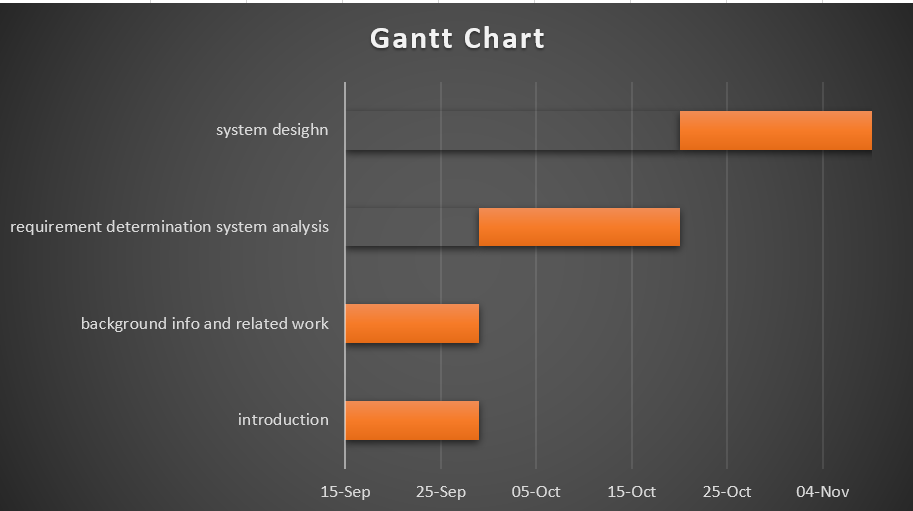
\includegraphics[width=\linewidth]{img/gantt_chart.png}
		\end{figure}
		\newpage	
		\chapter{Background Information \& Related Work}
			\section{Background Information}
			\subsection{IoT}
			\subsection{Hardware}
				\begin{itemize}
				\item \boldcolor{Raspberry Pi:} a small general purpose computer. All hardware components will be connected to it. An active connection to the internet is needed for it to fetch data from the server. %insert figure here% 
				\item \boldcolor{Ubuntu Web Server:} hosts the web application. Digital Ocean severs were chosen for this project.
				
				\item \boldcolor{LED:} since the hardware components controlled depends heavily on the user needs, this project main aim will be controlling a small LED. LED stands for light-emitting diode. Basically a small light source. %insert figure here% %
				\item \boldcolor{Linear Solenoid:} once the LED works, linear solenoid will be installed for demonstrating the idea. It is a small component that generates a linear motion. It will be used to press in anything, such as lights, TV remote, and coffee machine. %insert figure here%
				\end{itemize}
				
			\subsection{Programming Languages \& Frameworks}
				\begin{itemize}
					
					\item \boldcolor{Python:} raspberry pi can be controlled by either c++ or python. Python was chosen because a REST API can be made using it fast.
		 				\begin{itemize}
		 					\item \boldcolor{GPIO:} a library for controlling any hardware component connected to the GPIO pins.
		 					\item \boldcolor{Flask:} a lightweight framework to build web applications.
						\end{itemize}
					\item \boldcolor{Java:} mobile application are made in a native way with either swift or java.
						\begin{itemize}
							\item \boldcolor{Android:} a framework for making android apps.
							\item \boldcolor{Retrofit:} type-safe HTTP client for Android and Java. It will be used to send and receive commands and status from the web server.
							
						\end{itemize}
					\item \boldcolor{PostgreSQL:} an open-source RDBMS. It will be installed on the server.
				\end{itemize}
			
			\subsection{SDLC Model}
			\paragraph{} Incremental model will be used in this project. This model is a process of software development where requirements are broken down into multiple standalone modules of software development cycle. Incremental development is done in steps from analysis design, implementation, testing / verification, maintenance\cite{sdlc}. The reason this model was chosen is the pieces will be installed, tested and connected to the system gradually. First a LED, then a linear solenoid and so on.
			
			
		\newpage	
		\section{Related Work}
		\subsection{Insteon - Insteon Hub}
		\begin{figure}[H]
  			\caption{Related Work: Insteon}
			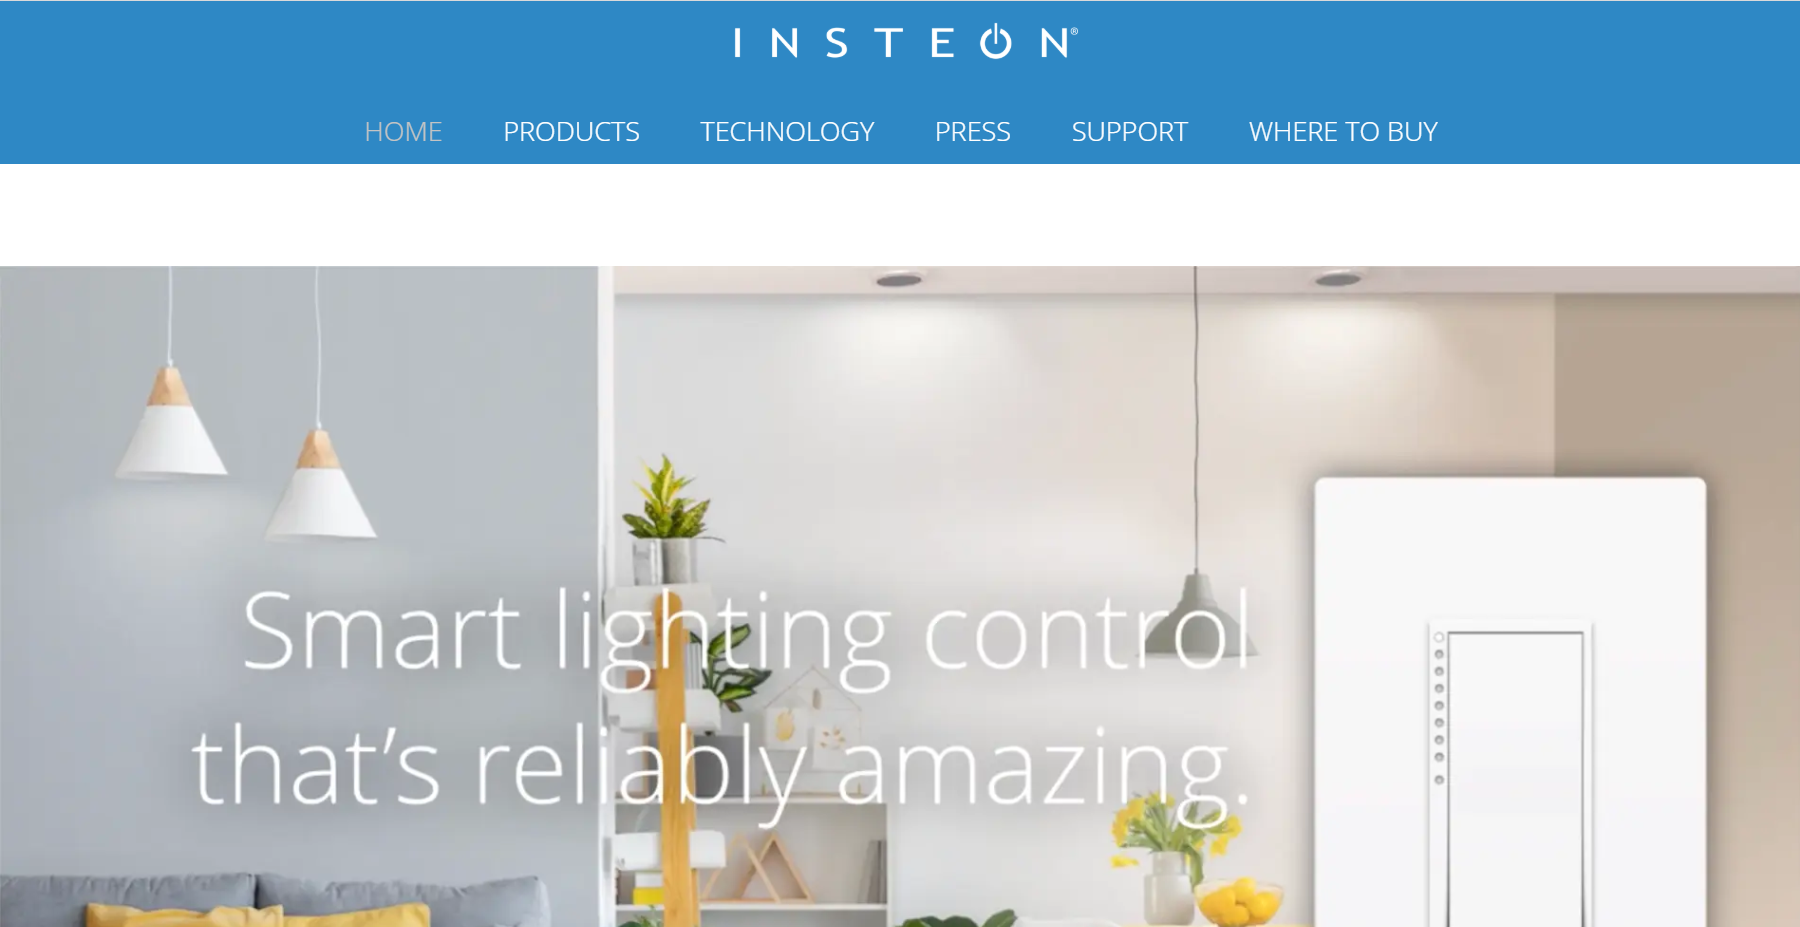
\includegraphics[width=\linewidth]{img/insteon.png}
		\end{figure}
		\paragraph{}Insteon Hub is a simple and straightforward device that connects you to your home from any smartphone or tablet, anywhere in the world. Control Insteon light bulbs, wall switches, outlets, and thermostats at home or remotely and receive instant email or push notification alerts from motion, door and window, water leak, and smoke sensors while you’re away. Homepage: \url{https://www.insteon.com/}
		\begin{itemize}
		\item \boldcolor{Advantage:}
			\begin{enumerate}
				\item Control Multiple Devices Simultaneously with a Basic Scene.
				\item Create Schedules to Turn Your Lights On and Off at Specific Times.
				\item Automatically Turn Lights On and Off with Sensors.
				\item Monitor Your Home with Email or Push Notification Alerts.
			\end{enumerate}
		\item \boldcolor{Disadvantage:} 
			\begin{enumerate}
				\item Hub setup takes a couple of minutes and a few moments per light switch, sensor.
				\item Its need to connect it to power and your home's internet router so if the internet die all devices need to start over again. 
				\item fixed the hub take more cost than its original price.
				\item There is no database save/restore. You have to recreate all the devices, scenes, schedules if its replaced.
			\end{enumerate}
		\end{itemize}
		\newpage	
		\subsection{Wink - Wink Hub 2}
		\begin{figure}[H]
  			\caption{Related Work: Wink}
  			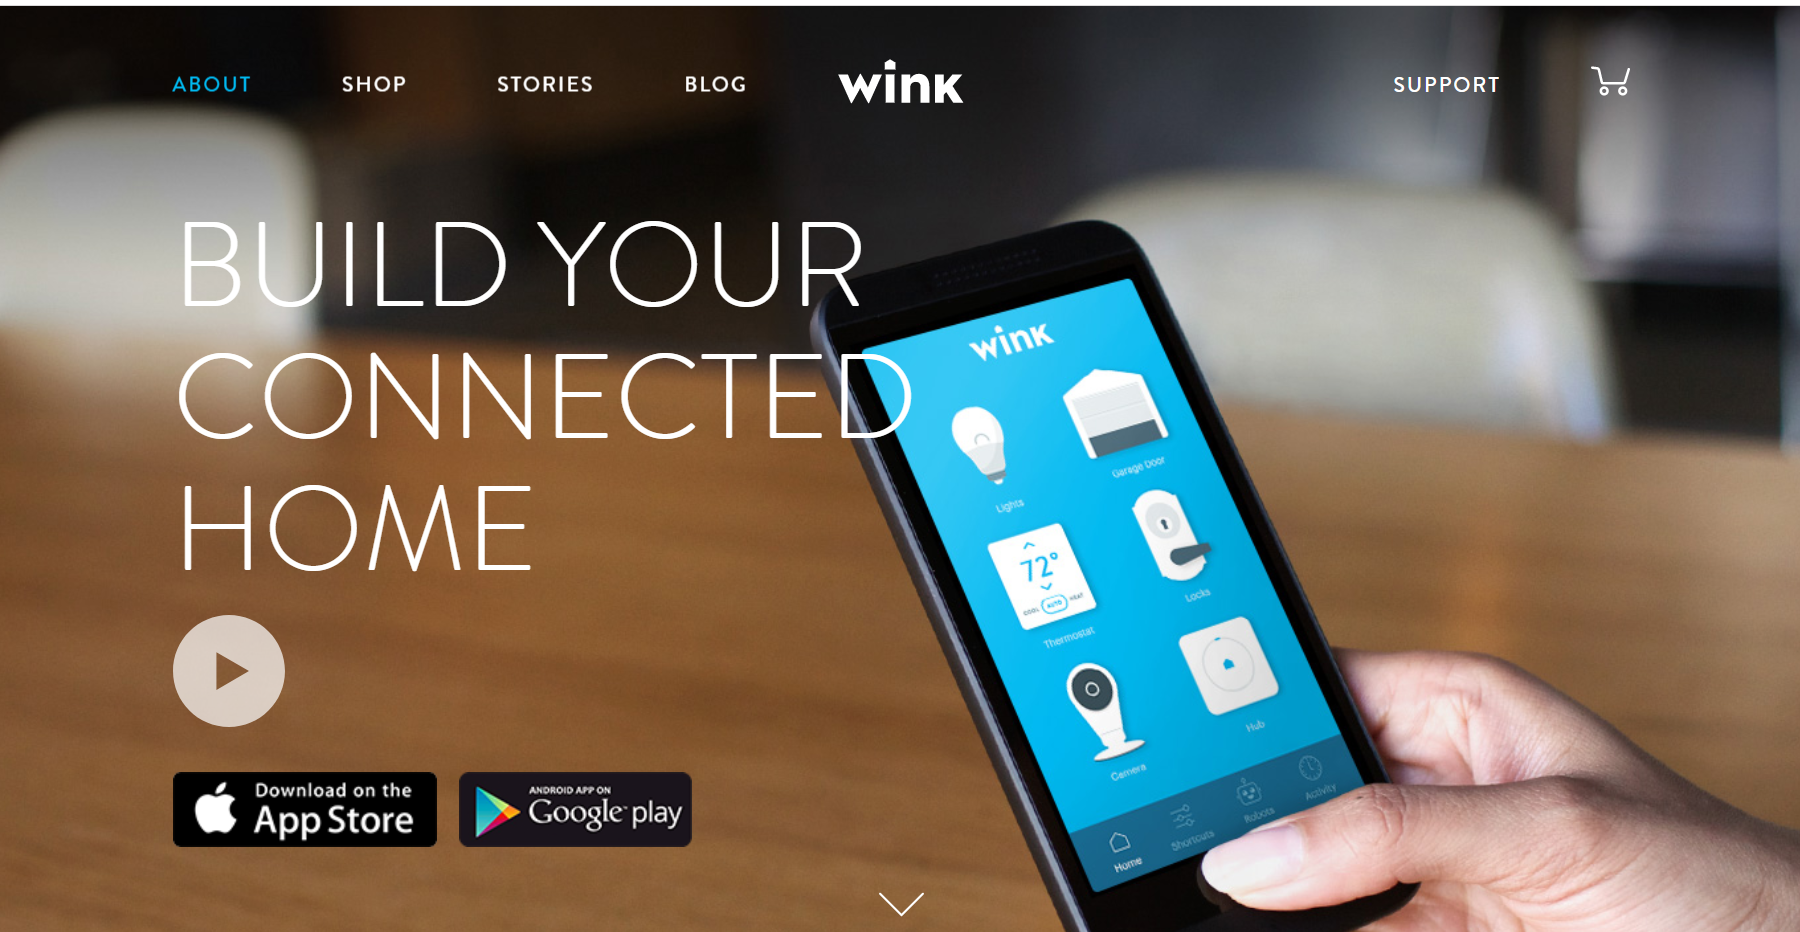
\includegraphics[width=\linewidth]{img/wink.png}
		\end{figure}
		\paragraph{}Wink Hub 2 is the world’s first smart home hub created for the mainstream consumer. With industry-leading smart home protocol support, enhanced connectivity features, and a sleek design, Wink Hub 2 brings hundreds of products from best-in-class brands together for a simple, intuitive experience. Home page: \url{https://www.wink.com/about/}
		
		\begin{itemize}
			\item \boldcolor{Advantage:}
			\begin{enumerate}
				\item Support Different platforms such as iOS or Android.
				\item Once you've created an account, Wink has the ability to recognize the products within Wink Bright, guide you through a few simple steps, and then you're ready to go.
				\item Wink works with Cortana Microsoft’s voice assistant and Amazon Alexa.
				\item One Important features in wink, its can see what you’re spending even before the bill arrives.
			\end{enumerate}
			\item \boldcolor{Disadvantage:} 
			\begin{enumerate}
				\item One major problem with the Wink 2 hub is that the device sometimes loses connectivity and must be reset in order for it to connect again.
				\item Wink app doesn't always let you access other devices' full features.
				\item High price.
				\item Takes 14 days to arrive.
			\end{enumerate}
		\end{itemize}
		\newpage
		\subsection{Samsung – Smart Things Hub}
		\begin{figure}[H]
  			\caption{Related Work: Samsung}
			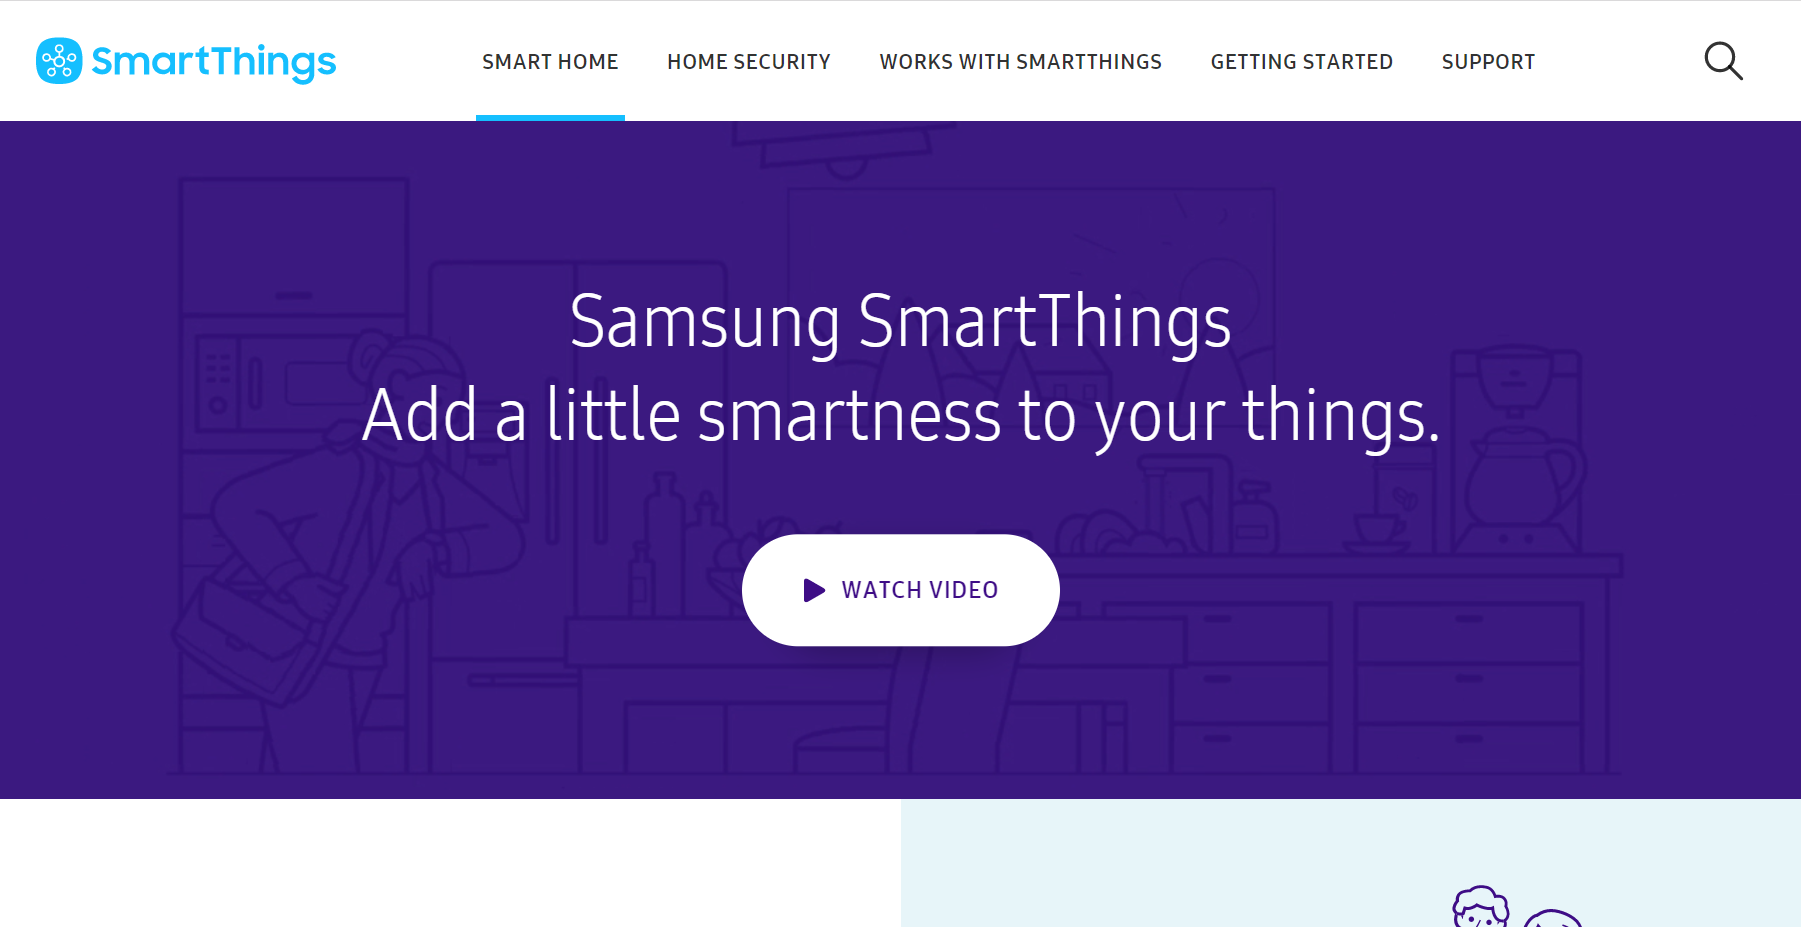
\includegraphics[width=\linewidth]{img/samsung.png}
		\end{figure}
		\paragraph{}Smart things hub Connect wirelessly with a wide range of smart devices and make them work together.
		Home page: \url{https://www.smartthings.com/}
		\begin{itemize}
			\item \boldcolor{Advantage:}
			\begin{enumerate}
				\item Monitor and control connected devices in your home using a single SmartThings app for iPhone or Android.
				\item Manage connected devices in your home with SmartThings Routines for Good Morning, Goodbye, Good Night, and more.
				\item Receive alerts from connected devices when there’s unexpected activity in your home.
				
			\end{enumerate}
			\item \boldcolor{Disadvantage:} 
			\begin{enumerate}
				\item Some compatible components may not work as efficiently or smoothly as you want them to, which may be inconvenient.
				\item Some users report it stops working at times.
				\item Difficult to upgrade from older hub.
				\item In US Only.
			\end{enumerate}
		\end{itemize}
		\section{Proposed \& Similar System Comparison}
			\def\arraystretch{1.5}
			\begin{table}[H]
				\caption{Proposed \& Similar System Comparison}
			\begin{center}
			\begin{tabularx}{\linewidth}{|m{4cm}*4{|X}|}\hline
					
					& \boldcolor{Raspberry Pi} & \boldcolor{Insteon} & \boldcolor{Wink hub 2} & \boldcolor{Samsung (smart things)}  \\\hline
					
					\boldcolor{design} &
						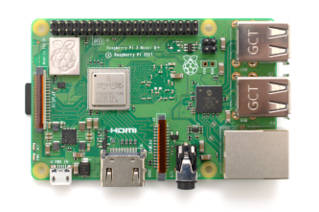
\includegraphics[width=\linewidth]{img/raspberry.png} &
						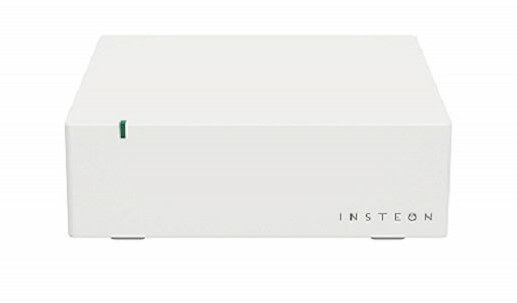
\includegraphics[width=\linewidth]{img/insteon_hw.png} & 
						\Includegraphics[width=\linewidth]{img/wink_hw.png} &
						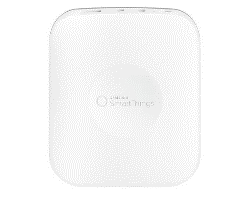
\includegraphics[width=\linewidth]{img/samsung_hw.png}
					 \\\hline
					\boldcolor{Works With Wi-Fi} & yes & yes & yes & yes  \\\hline


					
					\boldcolor{Parts Price} & very cheap & expensive & very expensive & expensive  \\\hline
					\boldcolor{Price} & 25\$ & 80\$ & 99\$ & 70\$ \\\hline
					
					\boldcolor{Installation \& Configuration Difficulty} & hard to install but doesn't takes time to reinstall and configure& easy to install and hardly takes any time setting up even if you change your home  & easy to install and hardly takes any time setting up even if you change your home  & easy to install and hardly takes any time setting up even if you change your home
					\\\hline
				\end{tabularx}
			\end{center}
		\end{table}
		\newpage	
		\begin{comment}
	\chapter{Requirement Determination \& Analysis}
		\section{System Analysis}
		\section{Gathering Information}
		\section{Requirement Specification}
			\subsection{Functional Requirements}
			\subsection{Non-Functional Requirements}
		\section{Requirement Analysis}
		\newpage	
	\chapter{System Design}
		\section{System Architecture}
		\section{User Interface Design}
		\newpage	
	\chapter{Implementation}
		\section{Implementation}
		\section{Implementation Requirements}
			\subsection{Software Requirements}
			\subsection{Hardware Requirements}
		\section{Implementation Detailed}
		\section{I/O Screens}
		\newpage	
	\chapter{Testing}
		\section{Testing}
		\section{Test Plan}
			\subsection{Unit Test}
			\subsection{Functional Test}
			\subsection{Acceptance Test}
		\section{Test Items}
			\subsection{Features to Be Tested}
			\subsection{Schedule of Test Actions}
			\subsection{Test Tasks}
		\section{Test Case}
		\section{Test Result}
		\newpage	
	\chapter{Conclusion}
		\section{Conclusion}
		\section{Evaluation}
		\section{Future Work}
	\newpage
	\end{comment}
	\addcontentsline{toc}{chapter}{References}
	\bibliographystyle{ieeetr}
	\bibliography{References}

	\addcontentsline{toc}{chapter}{Appendices}

\end{document}
